\renewcommand{\theequation}{\theenumi}
\renewcommand{\thefigure}{\theenumi}
\begin{enumerate}[label=\thesubsection.\arabic*.,ref=\thesubsection.\theenumi]
\numberwithin{equation}{enumi}
\numberwithin{figure}{enumi}

\item Find the distance between the pair of points (2,3) and (5,7). 
\\
\solution
\input{solutions/1/1/Assignment_2.tex}
\item 


\item 
\item 
Find the distance between the following pair of points
\begin{align}
\vec{A}&=\myvec{a\\0} & \vec{B}&=\myvec{0\\b}
\end{align}
\solution
		The distance between two vectors is given by 
\begin{align}
\label{1/4/eq5}
\norm{\vec{A}-\vec{B}}&= \sqrt{\myvec{\vec{A}-\vec{B}}^\top\myvec{\vec{A}-\vec{B}}}\\
\end{align}
$\because $
\begin{align}
\vec{A}-\vec{B}&=\myvec{a\\-b}
\\
\norm{\vec{A}-\vec{B}}&=\sqrt{\myvec{a & -b}\myvec{a\\-b}} \\
	&=\sqrt{\myvec{a^2+b^2}} 
\end{align}

\item 
Find the distance between the following pair of points
\begin{align}
\vec{A}&=\myvec{b+c\\c+a} & \vec{B}&=\myvec{c+a\\a+b}
\end{align}
\\
\solution
The distance between two vectors is given by 
\begin{align}
\label{1/5/eq:eq5}
\norm{\vec{A}-\vec{B}}&= \sqrt{\myvec{\vec{A}-\vec{B}}^\top\myvec{\vec{A}-\vec{B}}}\\
\end{align}
\begin{align}
	\because \vec{A}-\vec{B}&=\myvec{b+c\\c+a} -\myvec{c+a\\a+b}\\
&=\myvec{b-a\\c-b},
\end{align}
\begin{align}\brak{\vec{A}-\vec{B}}^{\top}\brak{\vec{A}-\vec{B}}
	&=\sqrt{\myvec{b-a & c-b}\myvec{b-a\\c-b}} \\
	&=\sqrt{\myvec{(b-a)^2+(c-b)^2}} 
\end{align}

\item 
\item 
Find the distance between the following pairs of points
\begin{align}
\myvec{am_1^2\\2am_1}, \myvec{am_2^2\\2am_2}
\end{align}
\\
\solution
	The distance between two vectors is given by 
\begin{align}
\norm{\vec{A}-\vec{B}}=\sqrt{\myvec{\vec{A}-\vec{B}}^
\top \myvec{\vec{A}-\vec{B}}}
\end{align}
Let $\vec{A}={\myvec{am_1^2\\2am_1}, \vec{B}=\myvec{am_2^2\\2am_2}}$
\begin{align}
\vec{A}-\vec{B}&=\myvec{am_1^2\\2am_1}-\myvec{am_2^2\\2am_2}
\\&=\myvec{am_1^2-am_2^2\\2am_1-2am_2}
\\&=a\myvec{m_1^2-m_2^2\\2\myvec{m_1-m_2}}
\\&=a\myvec{m_1-m_2}\myvec{m_1+m_2\\2}
\end{align}
by using the property of $\norm{k\vec{A}}=\abs{k} \,\norm{\vec{A}}$
\begin{align}
\norm{\vec{A}-\vec{B}}&=\norm{a\myvec{m_1-m_2}\myvec{m_1+m_2\\2}}
\end{align}
\begin{align}
=\abs{a\myvec{m_1-m_2}}\norm{\myvec{m_1+m_2\\2}}
\end{align}
\begin{align}
&=\abs{a\myvec{m_1-m_2}}\sqrt{\myvec{m_1+m_2\\2}^
\top\myvec{m_1+m_2\\2}}
\end{align}
\begin{align}
&=\abs{a\myvec{m_1-m_2}}\sqrt{\myvec{m_1+m_2&&2}\myvec{m_1+m_2\\2}}
\end{align}
\begin{align}
&=\abs{a\myvec{m_1-m_2}}\sqrt{\myvec{m_1+m_2}^2+\myvec{2}^2}\label{eq2}
\end{align}
\begin{align}
&=\abs{a\myvec{m_1-m_2}}\sqrt{\myvec{m_1+m_2}^2+4}
\end{align}
Distance between $(am_1^2,2am_1)$ and $(am_2^2,2am_2)$ is
\begin{align}
&=\abs{a\myvec{m_1-m_2}}\sqrt{\myvec{m_1+m_2}^2+4}
\end{align}

\item 
Find the distance between the following pairs of points
\begin{align}
\myvec{1\\-3}, \myvec{-2\\1}
\end{align}
\solution
	\begin{align}
\because \vec{A}-\vec{B} 
&=\myvec{1\\-3}-\myvec{-2\\1} \\
&=\myvec{3\\-4}, 
\label{1/8/eq5}
\end{align}
Hence, 
\begin{align}
\norm{\vec{A}-\vec{B}}&= \sqrt{\myvec{\vec{A}-\vec{B}}^\top\myvec{\vec{A}-\vec{B}}}\\
&=\sqrt{\myvec{3& -4} \myvec{3\\-4}} \\
&=\sqrt{3^2 + \myvec{-4}^2} \\
&=5 
\end{align}
\begin{figure}[!ht]
	\centering 
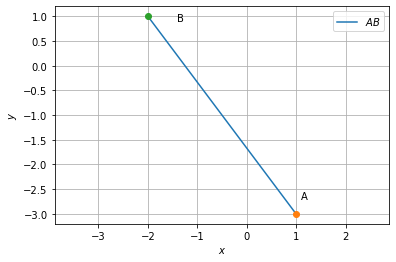
\includegraphics[width=\columnwidth]{solutions/1/8/diagram.png}
\caption{}
\label{1/8/fig:Line between A and B}
\end{figure}

\item 
\item 
A line of length 10 and one end is at point (2, -3); if the abscissa of the other end be 10, Prove that its ordinate must be 3 or -9.
\begin{align}
\myvec{2\\-3}, \myvec{10\\y_1} \label{1/10/eq:1}
\end{align}
\solution
%	\norm{\vec{A}-\vec{B}}=\sqrt{\myvec{\vec{A}-\vec{B}}^\intercal \myvec{\vec{A}-\vec{B}}} \label{1/10/eq:1.1}
\end{align}
Let
\begin{align}
\vec{A}&=\myvec{2\\-3}, \vec{B}=\myvec{10\\y_1} \nonumber    
\end{align}

\begin{align}
\\\vec{A-B}&=\myvec{-8\\-3-y_1}
\end{align}
Given Distance between $\vec{A}$ and $\vec{B}$ is 10
\\From \eqref{1/10/eq:1.1} & \eqref{1/10/eq:1}
\begin{align}
\norm{\myvec{-8\\-3-y_1}} &=10 \label{1/10/eq2}
\end{align}
\begin{align}
\sqrt{\myvec{-8\\-3-y_1}^\intercal\myvec{-8\\-3-y1}}&=10
\end{align}
\begin{align}
\sqrt{\myvec{-8&&-3-y_1}\myvec{-8\\-3-y_1}}&=10
\end{align}
\begin{align}
\sqrt{\myvec{-8}^2+\myvec{-3-y_1}^2}&=10
\end{align}
\begin{align}
\myvec{-8}^2+\myvec{-3-y_1}^2&=10^2
\end{align}
\begin{align}
64+9+6 y_1+y_1^2 &=100
\end{align}
\begin{align}
&=y_1^2+6y_1-27
\end{align}
On solving for $y_1$ in above quadratic equation
\begin{align}
\implies y_1=-6+\sqrt{144}, y_1=-6-\sqrt{144}
\end{align}
\begin{align}
\implies y_1=3, y_1=-9
\end{align}

\item 
\item 
\item 
\item 
\item 
\item 
Find coordinates of a point which divides the line joining the points (1, 3) and (2, 7) in the ratio 3 : 4
\\
\solution
		The point  dividing the line AB in the ratio $m:n$ is given by
\begin{align}
	\vec{P} &=\frac{m \vec{B} + n \vec{A}}{m + n}
\label{1/15eq5}
\end{align}
Let $\vec{A}=\myvec{1\\3}, \vec{B}=\myvec{2\\7}, {m}=3, {n}=4$\\
From \eqref{1/15eq5}
\begin{align}
&=\frac{3\myvec{2\\7}+4\myvec{1\\3}}{3 + 4}\\
&=\frac{\myvec{6\\21}+\myvec{4\\12}}{7}\\
&=\frac{\myvec{10\\33}}{7}\\
&=\myvec{\frac{10}{7}\\\frac{33}{7}}
\end{align}

\begin{figure}[!ht]
	\centering 
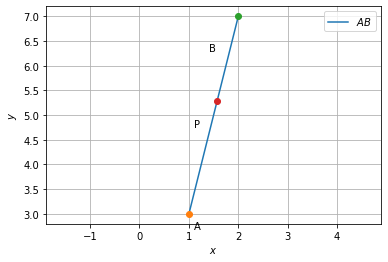
\includegraphics[width=\columnwidth]{solutions/1/15/assignment3.png}
\caption{}
\label{1/15fig:Dividing Line}
\end{figure}

 
\item 
\item 
Find coordinates of the point which divides, in-ternally and externally, the line joining (-1, 2) to (4,-5) in the ratio 2 : 3
\begin{align}
\vec{A}&=\myvec{-1\\2} & \vec{B}&=\myvec{4\\-5}
\end{align}
\solution
The coordinates of point $\vec{P}$, internally dividing the line AB in the ratio $m:n$ is given by
\begin{align}
\vec{P} &=\frac{m \vec{B} + n \vec{A}}{m + n}
\label{1/17/eq5}
\end{align}
Let $\vec{A}=\myvec{-1\\2}, \vec{B}=\myvec{4\\-5}, {m}=2, {n}=3$.

From \eqref{1/17/eq5}
\begin{align}
\vec{P}&=\frac{2\myvec{4\\-5}+3\myvec{-1\\2}}{2 + 3}\\
&=\myvec{1\\\frac{-4}{5}} 
\end{align}

The coordinates of point $\vec{Q}$, externally dividing the line AB in the ratio $m:n$ is given by\\
\begin{align}
\vec{Q}&=\frac{m \vec{B} - n \vec{A}}{m - n}
\label{1/17/eq6}
\end{align}
From \eqref{1/17/eq6}
\begin{align}
\vec{Q}&=\frac{2\myvec{4\\-5}-3\myvec{-1\\2}}{2 - 3}\\
&=\myvec{-11\\16 }
\end{align}
See Fig. 
\eqref{1/17/fig:Dividing Line}
\begin{figure}[!ht]
	\centering 
\includegraphics[width=\columnwidth]{solutions/1/17/assignment-4.png}
\caption{}
\label{1/17/fig:Dividing Line}
\end{figure}
 

\item Find the coordinates of the point which divides, internally and externally, the line joining (-3,-4) to (-8,7) in the ratio 7:5
\\
\solution

Let
\begin{align}
    \Vec{A}=\myvec{-3\\-4}
\end{align}
\begin{align}
    \Vec{B}=\myvec{-8\\7}
\end{align}
\begin{enumerate}
\item Using section formula for internal division, 
\begin{align}
\vec{S}&=\large{\frac{7\myvec{-8\\7}+5\myvec{-3\\-4}}{\brak{7+5}}}   
\\
&=\frac{1}{12}\myvec{{-71} \\ {29}}
\end{align}
\item Similarly, for external division, 
\begin{align}
\vec{S}&=\large{\frac{7\myvec{-8\\7}-5\myvec{-3\\-4}}{\brak{7-5}}}   
&=\frac{1}{2} \myvec{{-41} \\ {69}}
\end{align}

Fig. \ref{1/18fig} plots the desired points.
\begin{figure}[!ht]
\centering
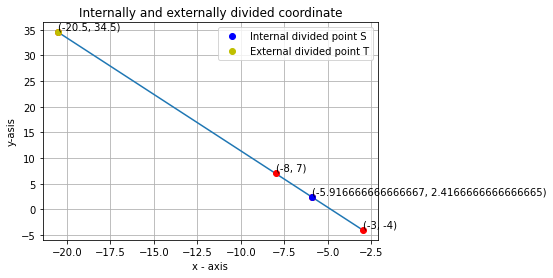
\includegraphics[width=\columnwidth]{solutions/1/18/Internal and external point.png}
\caption{ Plot of coordinate of the point which divides internally and externally }
\label{1/18fig}
\end{figure}
 \end{enumerate} 
 
%
\item The line joining the points (1, -2) and (-3,4) is  trisected;Find the coordinates of the points of the trisection.
\\
\solution
Let 
%
\begin{align}
    \Vec{A}=\myvec{1\\-2},
    \Vec{B}=\myvec{-3\\4}
\end{align}
%
Then, 
\begin{align}
\vec{Q}&=\frac{2\myvec{-3\\4}+1\myvec{1\\-2}}{\brak{1+2}}   \\
&
=\myvec{\frac{-5}{3}\\[0.2cm]{2}}
\\
\vec{P}&=\frac{1\myvec{-5/3\\2}+1\myvec{1\\-2}}{\brak{1+1}}   
\\
&=\myvec{\frac{-1}{3} \\[0.2cm]{0}}
\end{align}
Fig. \ref{1/19/python fig1.png} verifies the result.
\begin{figure}[!ht]
\centering
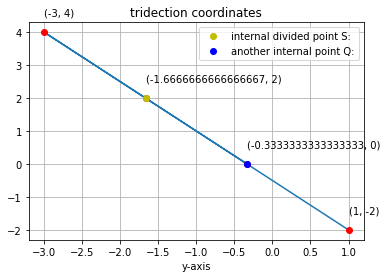
\includegraphics[width=\columnwidth]{solutions/1/19/assignment.1.pythom plot.png}
\caption{ Plot of coordinates}
\label{1/19/python fig1.png}
\end{figure}


 

\item 
\item 
\item 
\item 
\item 
\item 
\item 
\item 
\item 
\item 
\item 
\item 
\item 
% \item The coordinates of the vertices of a triangle are $(x_1,y_1)$, $(x_2,y_2)$ and $(x_3,y_3)$. The line joining the first two is divided in the ratio $l:k$, and the line joining his point of division to the opposite angular point is then divided in the ratio  $m:k+l$. Find the coordinates of the latter point of section. 
% %
% \\
% \solution
% \From elementary analysis of coordinate geometry and in view of Fig.\ref{eq:solutions/2/22/f2}, as $\bf{D}$ divides the line AB in the ratio $AD:DC=l:k$, we have:

\begin{equation}
 {\bf{D}}=\frac{l{\bf{B}}+k\bf{A}}{l+k}
    \label{eq:solutions/2/22/eq4}
\end{equation}
The position vector $\bf{E}$ which  divides CD in the ratio $DE:EC=m:l+k$,  is clearly obtained by setting $l=m,k=l+k,\bf{A=D,B=C}$ and is given by: 

\begin{equation}
 {\bf{E}}=\frac{m{\bf{C}}+(l+k)\bf{D}}{m+l+k}
    \label{eq:solutions/2/22/eq5}
\end{equation}
 
Using Eq.\ref{eq:solutions/2/22/eq4} into Eq.\ref{eq:solutions/2/22/eq5} and simplifying yields :
\begin{equation}
 {\bf{E}}=\frac{m {\bf{C}}+l{\bf{B}}+k{\bf{A}}}{m+l+k}
    \label{eq:solutions/2/22/eq6}
\end{equation}

Where,
%\begin{align}
 $  \bf{A}  = \begin{pmatrix}
           x_{1} \\
           y_{1} \\
         \end{pmatrix}$, $ \bf{B}  = \begin{pmatrix}
           x_{2} \\
           y_{2} \\
         \end{pmatrix}$  and $  \bf{C}  = \begin{pmatrix}
           x_{3} \\
           y_{3} \\
         \end{pmatrix}$
         
In Fig.\ref{eq:solutions/2/22/f2}, the solution obtained from the Python code is depicted for a particular choice of input viz. $l=1,m=1,k=1$ and $A(0,0),B(3,3)\, $\&$\, C(6,0)$.
Using, Eq.\ref{eq:solutions/2/22/eq6} and the above mentioned input, we have:

$  \bf{E}  = \begin{pmatrix}
           x_{E} \\
           y_{E} \\
         \end{pmatrix}$ $=\begin{pmatrix}
           3 \\
           1 \\
         \end{pmatrix}$



 \begin{figure}[!ht]
    \centering
    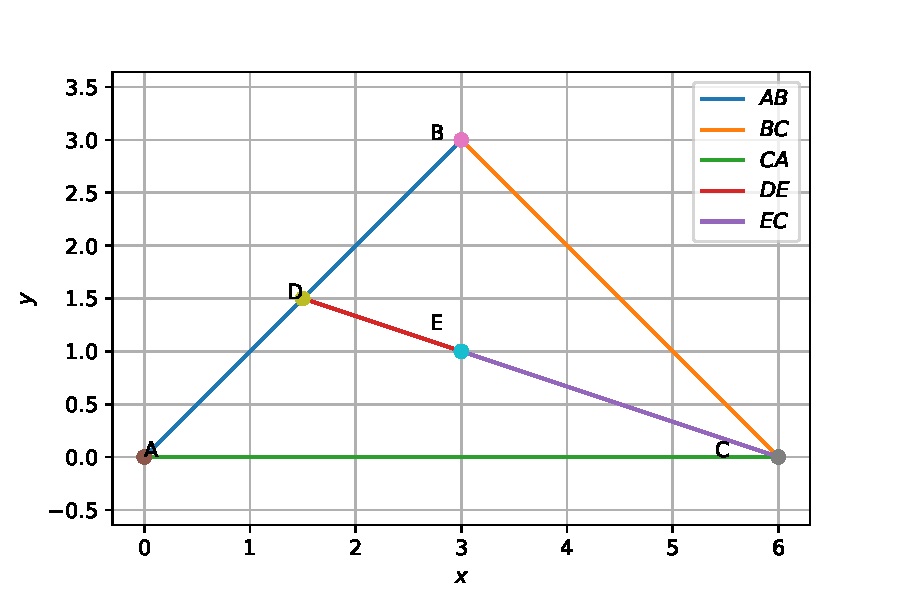
\includegraphics[width=\columnwidth]{./solutions/2/22/Ex1prob22.pdf}
    \caption{For $l=1,m=1,k=1$ and $A(0,0),B(3,3)\, $\&$\, C(6,0)$, the solution $E(3,1)$ is obtained using Python}
    \label{eq:solutions/2/22/f2}
\end{figure}
       


\end{enumerate}
